\section{Embedded Linux application development}

\begin{frame}{Contents}
  \begin{itemize}
  \item Application development
    \begin{itemize}
    \item Developing applications on embedded Linux
    \item Building your applications
    \end{itemize}
  \item Debugging and analysis tools
    \begin{itemize}
    \item Debuggers
    \item Remote debugging
    \item Tracing and profiling
    \end{itemize}
  \end{itemize}
\end{frame}

\subsection{Developing applications on embedded Linux}

\begin{frame}{Application development}
  \begin{itemize}
  \item An embedded Linux system is just a normal Linux system, with
    usually a smaller selection of components
  \item In terms of application development, developing on embedded
    Linux is exactly the same as developing on a desktop Linux system
  \item All existing skills can be re-used, without any particular
    adaptation
  \item All existing libraries, either third-party or in-house, can be
    integrated into the embedded Linux system
    \begin{itemize}
    \item Taking into account, of course, the limitation of the
      embedded systems in terms of performance, storage and memory
    \end{itemize}
  \item Application development could start on x86, even before
      the hardware is available.
  \end{itemize}
\end{frame}

\begin{frame}{Leverage existing libraries and languages}
  \begin{itemize}
  \item Many developers getting started with embedded Linux limit
    themselves to C, sometimes C++, and the C/C++ standard library.
  \item However, there are a lot of libraries and languages that can
    help you accelerate and simplify your application development
    \begin{itemize}
    \item Compiled languages like Rust and Go are increasingly popular
    \item Interpreted languages, especially Python
    \item Higher-level libraries: Qt, Glib, Boost, and many more
    \end{itemize}
  \item Make sure to evaluate what is the right choice for your
    project, but pay attention it
    \begin{itemize}
    \item Footprint and performance on low-end platforms
    \item Use well-maintained and well-known technologies
    \end{itemize}
  \end{itemize}
\end{frame}

\begin{frame}{Building your applications/libraries}
  \begin{itemize}
  \item Even for simple applications or libraries, make use of a build
    system
    \begin{itemize}
    \item \href{https://cmake.org/}{CMake}
    \item \href{https://mesonbuild.com/}{Meson}
    \end{itemize}
  \item This will simplify
    \begin{itemize}
    \item the build process of your application
    \item the life of developers joining your project
    \item the packaging of your application into an embedded Linux
      build system
    \end{itemize}
  \end{itemize}
\end{frame}

\begin{frame}[fragile]{Getting started with {\em meson}}
  \begin{block}{Minimal {\tt meson.build}}
\begin{verbatim}
project('example', 'c')
executable('demo', 'main.c')
\end{verbatim}
  \end{block}

  \begin{block}{{\tt meson.build} for multiple programs and source files}
\begin{verbatim}
project('example', 'c')
src_demo1 = ['demo1.c', 'foo1.c']
executable('demo1', src_demo1)
src_demo2 = ['demo2.c', 'foo2.c']
executable('demo2, src_demo2)
\end{verbatim}
  \end{block}
\end{frame}

\begin{frame}[fragile]{Options with {\em meson}}
  \begin{block}{{\tt meson\_options.txt}}
\begin{verbatim}
option('demo-debug', type : 'feature', value : 'disabled')
\end{verbatim}
  \end{block}

  \begin{block}{{\tt meson.build}}
\begin{verbatim}
project('tutorial', 'c')
demo_c_args = []
if get_option('demo-debug').enabled()
   demo_c_args += '-DDEBUG'
endif
executable('demo', 'main.c', c_args: demo_c_args)
\end{verbatim}
  \end{block}
\end{frame}

\begin{frame}[fragile]{Library dependencies with {\em meson}}
  \begin{block}{{\tt meson.build}}
\begin{verbatim}
project('tutorial', 'c')
gtkdep = dependency('gtk+-3.0')
executable('demo', 'main.c', dependencies : gtkdep)
\end{verbatim}
  \end{block}

  The dependency \code{gtk+-3.0} is searched using \code{pkg-config}.
\end{frame}

\subsection{Debugging}

\begin{frame}{GDB}
  \begin{itemize}
  \item GDB: {\bf GNU Debugger}
  \item The reference debugger on Linux
  \item Supports most embedded architectures
  \item Source-level debugger: C, C++, Pascal, Objective-C, Fortran,
    Ada...
  \item Console interface, but integration in many graphical IDEs
  \item Can be used to
    \begin{itemize}
    \item control the execution of a running program
    \item analyze post mortem a program crash
    \end{itemize}
  \item Needs program and libraries compiled with {\em debugging
      symbols}, using gcc \code{-g} option
  \item \url{https://www.gnu.org/software/gdb/}
  \item \href{https://www.youtube.com/watch?v=JGhAgd2a_Ck}{Tutorial:
      Debugging Embedded Devices using GDB}
  \end{itemize}
\end{frame}

\begin{frame}[fragile]{GDB crash course (1)}
  \begin{itemize}
  \item Example for {\em native debugging}
    \begin{itemize}
    \item \code{gdb} runs on the same machine as the program to debug
    \end{itemize}
  \item Compile with debugging symbols, for example with {\em meson}
    \begin{block}{}
      {\small
\begin{verbatim}
$ meson -Ddebug=true
$ ninja
$ file test
test: LF 64-bit LSB executable, x86-64, [...], with debug_info
\end{verbatim}
      }
    \end{block}
  \item Start {\em gdb} with the program as argument, {\em gdb} loads
    the debugging symbols and waits at its prompt
    \begin{block}{}
      {\small
\begin{verbatim}
$ gdb test
GNU gdb (GDB) Fedora 12.1-1.fc36
[...]
Reading symbols from test...
(gdb)
\end{verbatim}
      }
    \end{block}
  \end{itemize}
\end{frame}

\begin{frame}{GDB crash course (2)}
  \begin{itemize}
  \item \code{help}\\
    Get some useful help!
  \item \code{break foobar} (\code{b})\\
    Set a breakpoint at the entry of function \code{foobar()}
  \item \code{break foobar.c:42}\\
    Set a breakpoint in \code{foobar.c}, line 42
  \item \code{print var} or \code{print task->files[0].fd} (\code{p})\\
    Print the variable \code{var}, or a more complicated reference. GDB
    can also nicely display structures with all their members
  \end{itemize}
\end{frame}

\begin{frame}{GDB crash course (3)}
  \begin{itemize}
  \item \code{continue} (\code{c})\\
    Continue the execution after a breakpoint
  \item \code{next} (\code{n})\\
    Continue to the next line, stepping over function calls
  \item \code{step} (\code{s})\\
    Continue to the next line, entering into subfunctions
  \item \code{backtrace} (\code{bt})\\
    Display the program stack
  \end{itemize}
\end{frame}

\subsection{Remote debugging}

\begin{frame}{Remote debugging}
  \begin{itemize}
  \item In a non-embedded environment, debugging takes place using \code{gdb}
    or one of its front-ends.
    \begin{itemize}
    \item \code{gdb} has local access to the binary and libraries compiled
      with debugging symbols
    \end{itemize}
  \item However, in an embedded context, the target platform
    environment is often too limited
    \begin{itemize}
    \item \code{gdb} itself is a bit large
    \item but more importantly, debugging symbols can be extremely large
    \end{itemize}
  \item Remote debugging is preferred
    \begin{itemize}
    \item \code{ARCH-linux-gdb} is used on the development workstation, offering
      all its features.
    \item \code{gdbserver} is used on the target system (only 100 KB
      on arm).
    \end{itemize}
  \end{itemize}
  \begin{center}
    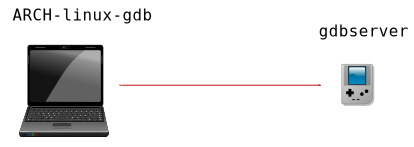
\includegraphics[width=0.5\textwidth]{slides/sysdev-application-development/gdb-vs-gdbserver.pdf}
  \end{center}
\end{frame}

\begin{frame}{Remote debugging: architecture}
  \begin{center}
    \includegraphics[width=\textwidth]{slides/sysdev-application-development/gdb-vs-gdbserver-architecture.pdf}
  \end{center}
\end{frame}

\begin{frame}{Remote debugging: on the target}
  \begin{itemize}
  \item Start the program through \code{gdbserver}
    \begin{itemize}
    \item TCP socket communication: \code{gdbserver localhost:<port> <executable> <args>}
    \item Serial port communication: \code{gdbserver /dev/ttyS0 <executable> <args>}
    \item {\em gdbserver} does not start the program, it waits for
      {\em gdb} to connect and start the program
    \end{itemize}
  \item Attach \code{gdbserver} to an already running program, using
    its PID
    \begin{itemize}
    \item \code{gdbserver --attach localhost:<port> <pid>}
    \end{itemize}
  \end{itemize}
\end{frame}

\begin{frame}{Remote debugging: on the host}
  \begin{itemize}
  \item Start \code{ARCH-linux-gdb <executable>}
  \item Then use the following \code{gdb} commands:
    \begin{itemize}
    \item To connect to the target:\\
      \code{gdb> target remote <ip-addr>:<port>} (networking)\\
      \code{gdb> target remote /dev/ttyUSB0} (serial link)
    \item To tell \code{gdb} where shared libraries are:\\
      \code{gdb> set sysroot <library-path>} (without \code{lib/})
    \end{itemize}
  \end{itemize}
\end{frame}

\begin{frame}{Post mortem analysis}
  \begin{itemize}
  \item When an application crashes due to a {\em segmentation fault}
    and the application was not under control of a debugger, we get no
    information about the crash
  \item Fortunately, Linux can generate a \code{core} file that
    contains the image of the application memory at the moment of the
    crash, and gdb can use this \code{core} file to let us analyze the
    state of the crashed application
  \item On the target
    \begin{itemize}
    \item Use \code{ulimit -c unlimited} in the shell starting the
    application, to enable the generation of a \code{core} file
    when a crash occurs
    \end{itemize}
  \item On the host
    \begin{itemize}
    \item After the crash, transfer the \code{core} file from the target to
      the host, and run
      \code{ARCH-linux-gdb -c core-file application-binary}
    \end{itemize}
  \end{itemize}
\end{frame}

\subsection{Tracing and profiling}

\begin{frame}[fragile]
  \frametitle{strace}
  \begin{columns}
  \column{0.75\textwidth}
  \small
  System call tracer - \url{https://strace.io}
  \begin{itemize}
  \item Available on all GNU/Linux systems\\
        Can be built by your cross-compiling toolchain generator or by your build system.
  \item Allows to see what any of your processes is doing: accessing files, allocating memory...
        Often sufficient to find simple bugs.
  \item Usage:\\
    \code{strace <command>} (starting a new process)\\
    \code{strace -p <pid>} (tracing an existing process)\\
    \code{strace -c <command>} (statistics of system calls taking most time)
  \end{itemize}
  See \href{https://man7.org/linux/man-pages/man1/strace.1.html}{the strace manual} for details.
  \column{0.25\textwidth}
  \includegraphics[height=0.7\textheight]{common/strace-mascot.png}\\
  \tiny Image credits: \url{https://strace.io/}
  \end{columns}
\end{frame}

\begin{frame}[fragile]
  \frametitle{strace example output}
  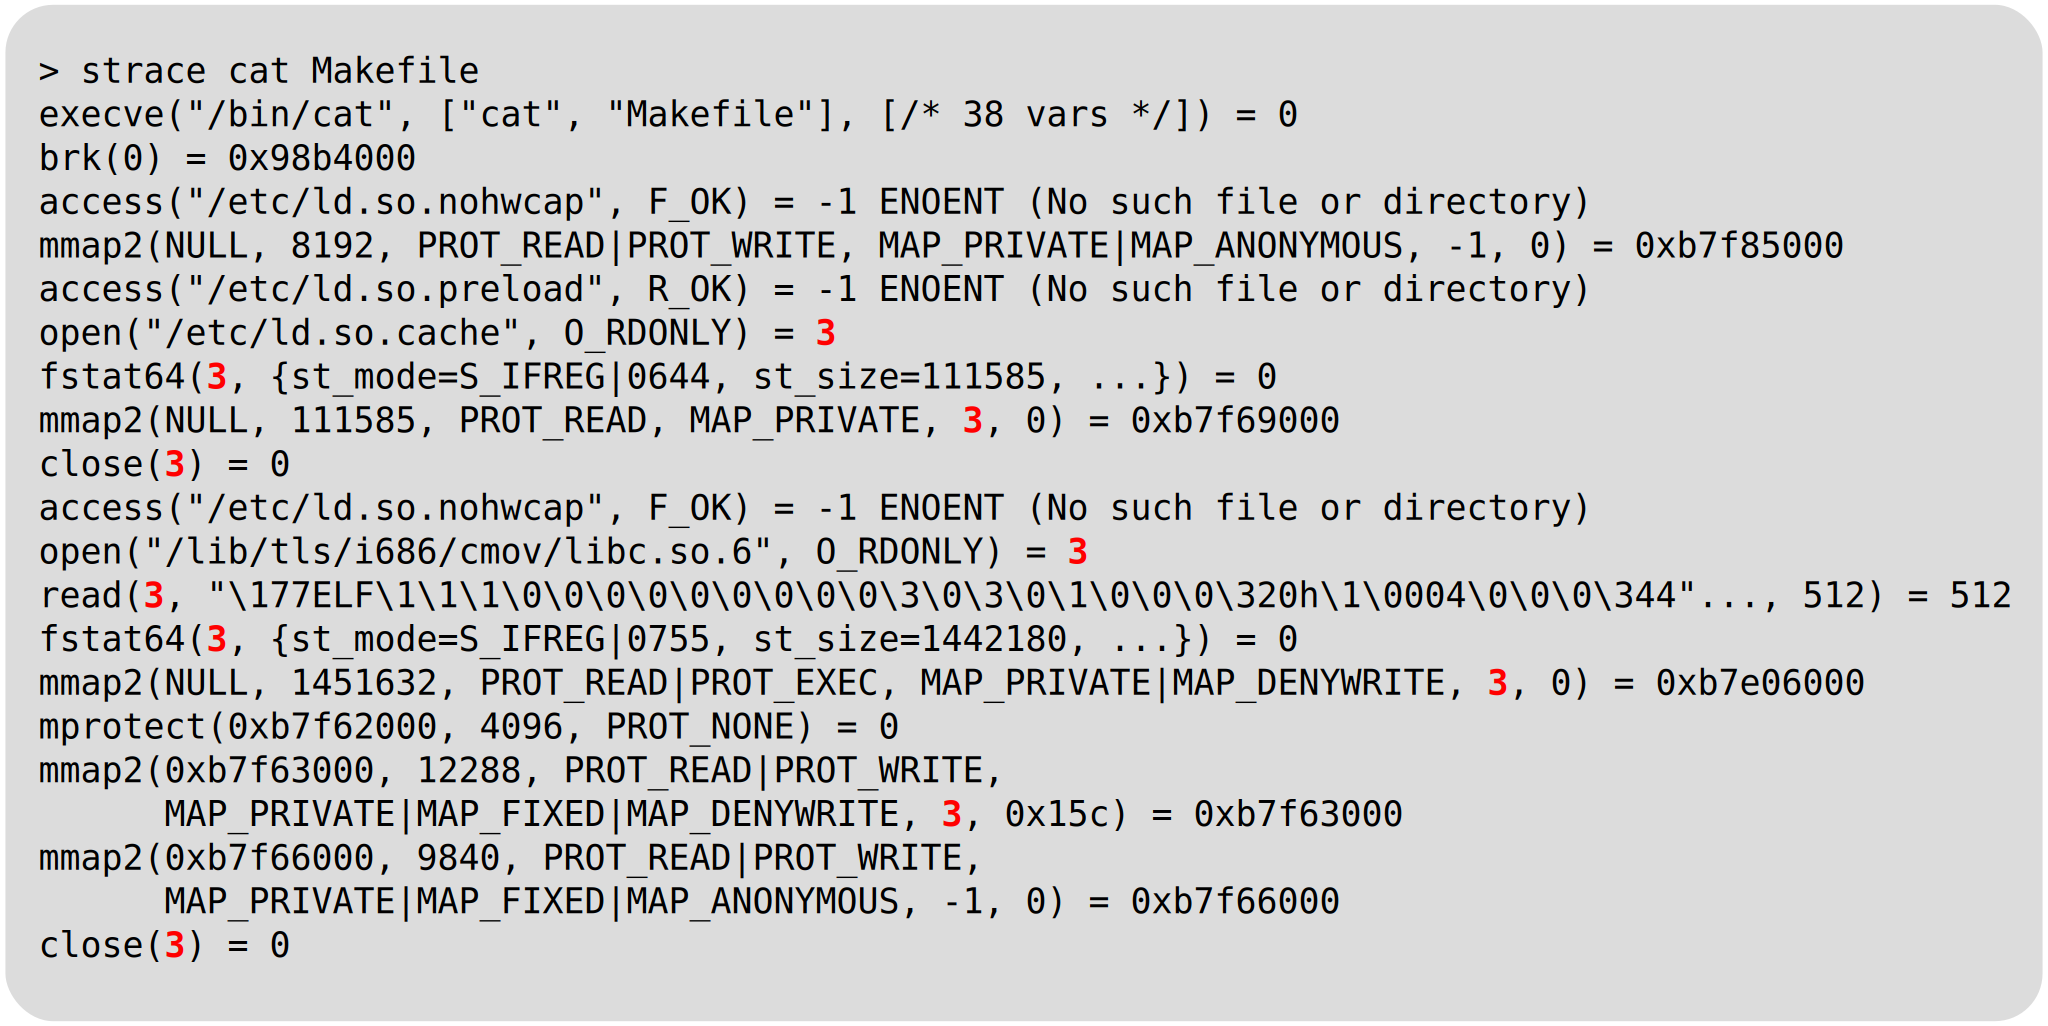
\includegraphics[height=0.75\textheight]{common/strace-output.pdf}\\
  Hint: follow the open file descriptors returned by \code{open()}.
  This tells you what files are handled by further system calls.
\end{frame}

\begin{frame}[fragile]
  \frametitle{strace -c example output}
  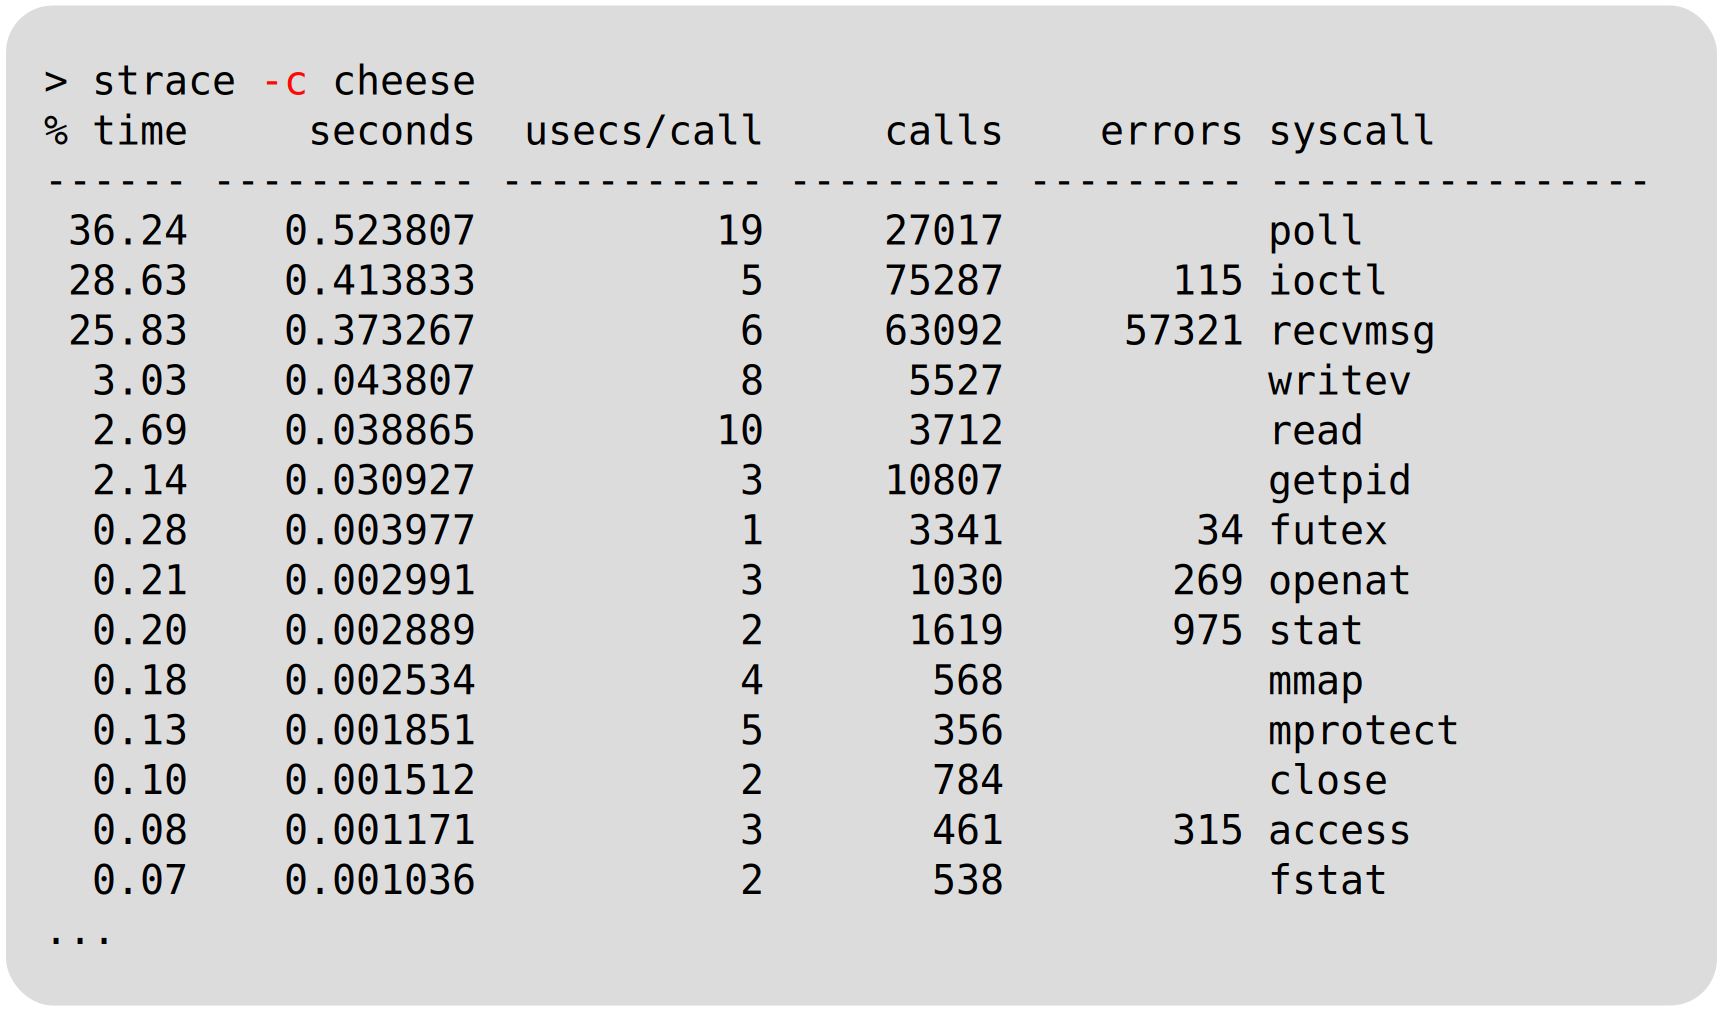
\includegraphics[height=0.8\textheight]{common/strace-c-output.pdf}
\end{frame}

\begin{frame}
  \frametitle{ltrace}
  A tool to trace library calls used by a program and all the signals
  it receives
  \begin{itemize}
  \item Very useful complement to \code{strace}, which shows only system
    calls. Library calls include system calls too!
  \item Of course, works even if you don't have the sources
  \item Allows to filter library calls with regular expressions, or
    just by a list of function names.
  \item Also offers a summary with its \code{-c} option.
  \item Manual page: \url{https://linux.die.net/man/1/ltrace}
  \item Works better with {\em glibc}. \code{ltrace} was broken
        with {\em uClibc} and may still be.
  \end{itemize}
  See \url{https://en.wikipedia.org/wiki/Ltrace} for details
\end{frame}

\begin{frame}[fragile]
  \frametitle{ltrace example output}
  \small
  \begin{block}{}
\begin{verbatim}
ltrace nedit index.html
sscanf(0x8274af1, 0x8132618, 0x8248640, 0xbfaadfe8, 0) = 1
sprintf("const 0", "const %d", 0) = 7
strcmp("startScan", "const 0") = 1
strcmp("ScanDistance", "const 0") = -1
strcmp("const 200", "const 0") = 1
strcmp("$list_dialog_button", "const 0") = -1
strcmp("$shell_cmd_status", "const 0") = -1
strcmp("$read_status", "const 0") = -1
strcmp("$search_end", "const 0") = -1
strcmp("$string_dialog_button", "const 0") = -1
strcmp("$rangeset_list", "const 0") = -1
strcmp("$calltip_ID", "const 0") = -1
\end{verbatim}
\end{block}
\end{frame}


\begin{frame}{ftrace}
  \begin{itemize}
  \item In-kernel {\em tracing} functionality
  \item Can trace
    \begin{itemize}
    \item Well-defined trace locations in the kernel, called {\em
        tracepoints}, identifying important events in the kernel:
      scheduling, interrupts, etc.
    \item Arbitrary functions in the kernel
    \item Arbitrary functions in user-space applications
    \end{itemize}
  \item Low-overhead and optimized tracing
  \item Accessible using the dedicated {\em tracefs} filesystem
  \item \code{trace-cmd} is a higher-level CLI tool to use {\em
      ftrace}
  \item Can be used to understand overall system activity (what is my
    system doing?) as well as narrow down specific performance
    issues
  \item \url{https://www.kernel.org/doc/Documentation/trace/ftrace.txt}
  \item \url{https://www.trace-cmd.org/}
  \end{itemize}
\end{frame}

\begin{frame}{kernelshark}
  \begin{itemize}
  \item Visualization tool for {\em ftrace} traces
  \item \url{https://kernelshark.org/}
  \end{itemize}
  \begin{center}
    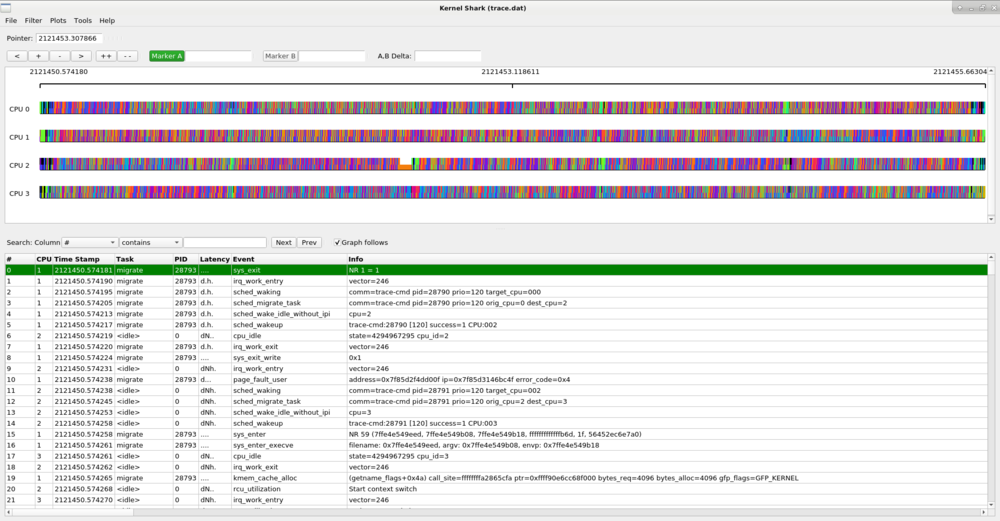
\includegraphics[height=0.6\textheight]{slides/sysdev-application-development/kernelshark.png}
  \end{center}
\end{frame}

\begin{frame}{perf}
  \begin{itemize}
  \item {\em instrument CPU performance counters, tracepoints, kprobes, and uprobes}
  \item Directly included in the Linux kernel source code: \kfile{tools/perf}
  \item Began as a tool for using the performance counters in Linux,
    and has had various enhancements to add tracing capabilities
  \item Supports a list of measurable events: hardware events (cycle
    count, L1 cache hits/miss, page faults), software events
    (tracepoints)
  \item \url{https://perf.wiki.kernel.org}
  \end{itemize}
\end{frame}

\begin{frame}{perf examples}
  \begin{itemize}
  \item List all currently known events\\
    \code{perf list}
  \item List scheduler tracepoints\\
    \code{perf list 'sched:*'}
  \item CPU counter statistics for the specified command\\
    \code{perf stat <command>}
  \item CPU counter statistics for the entire system, for 5 seconds\\
    \code{perf stat -a sleep 5}
  \item Profiling: sample on-CPU functions for the specified command, at 99 Hertz\\
    \code{perf record -F 99 <command>}
  \item Tracing: trace all context-switches via sched tracepoint, until Ctrl-C\\
    \code{perf record -e sched:sched_switch -a}
  \item Many more at \url{https://www.brendangregg.com/perf.html}
  \end{itemize}
\end{frame}

\begin{frame}{perf GUI: hotspot}
  \begin{columns}
    \column{0.4\textwidth}
    \begin{itemize}
    \item Hotspot - the Linux perf GUI for performance analysis
    \item The main feature of hotspot is visualizing a \code{perf.data} file graphically
    \item \href{https://github.com/KDAB/hotspot}{github.com/KDAB/hotspot}
    \end{itemize}
    \column{0.6\textwidth}
    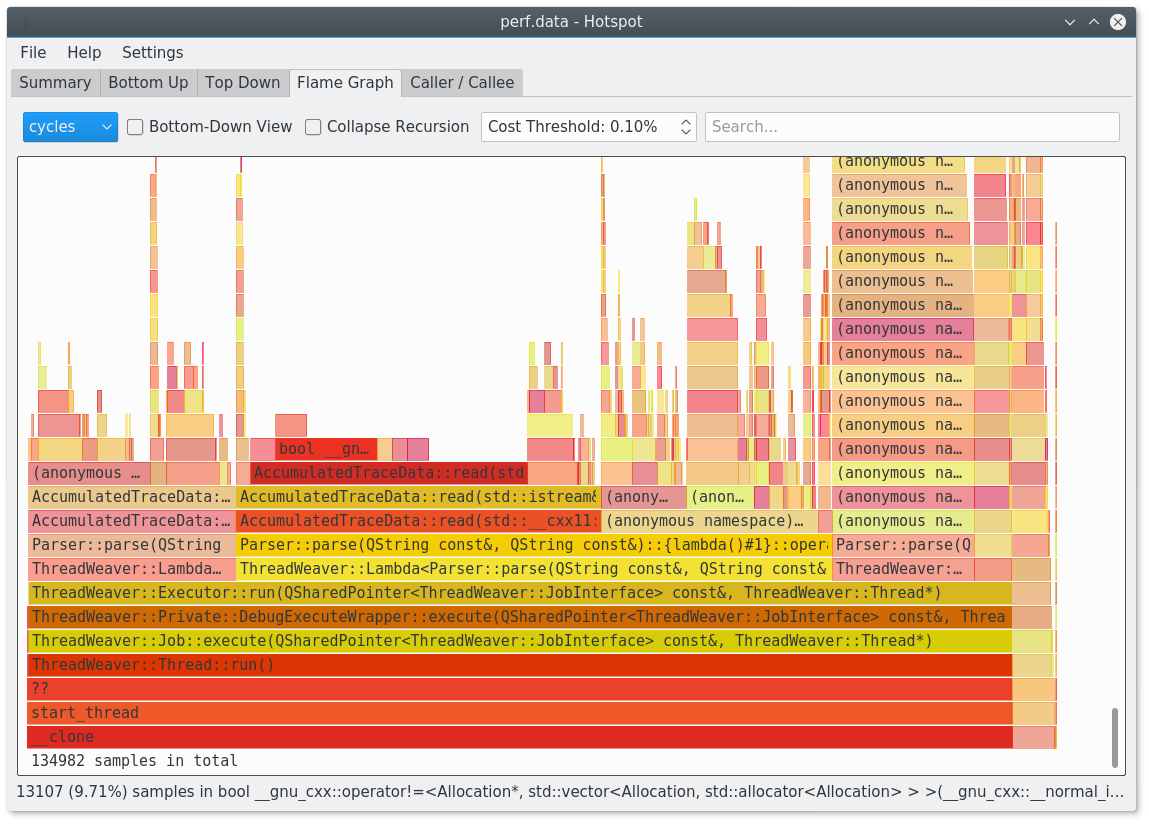
\includegraphics[width=\textwidth]{slides/sysdev-application-development/hotspot.png}
  \end{columns}
\end{frame}

\begin{frame}{gprof}
  \begin{itemize}
  \item Application-level profiler
  \item Part of {\em binutils}
  \item Requires passing gcc \code{-pg} option at build/link time
  \item Run your program normally, it automatically generates a
    \code{gmon.out} file when exiting
  \item Use the \code{gprof} tool on \code{gmon.out} to extract
    profiling data
  \item \url{http://sourceware.org/binutils/docs/gprof/}
  \end{itemize}
\end{frame}

\begin{frame}[fragile]{gprof example}
  \begin{columns}
    \column{0.6\textwidth}
    \begin{block}{}
      {\tiny
\begin{verbatim}
$ ./test-gprof
$ gprof test-gprof gmon.out
Flat profile:

Each sample counts as 0.01 seconds.
  %   cumulative   self              self     total
 time   seconds   seconds    calls   s/call   s/call  name
 35.31      7.46     7.46        1     7.46    13.92  func1
 34.03     14.65     7.19        1     7.19     7.19  func2
 30.57     21.11     6.46        1     6.46     6.46  new_func1
  0.09     21.13     0.02                             main
[...]
\end{verbatim}
      }
    \end{block}
    \column{0.4\textwidth}
    \begin{center}
      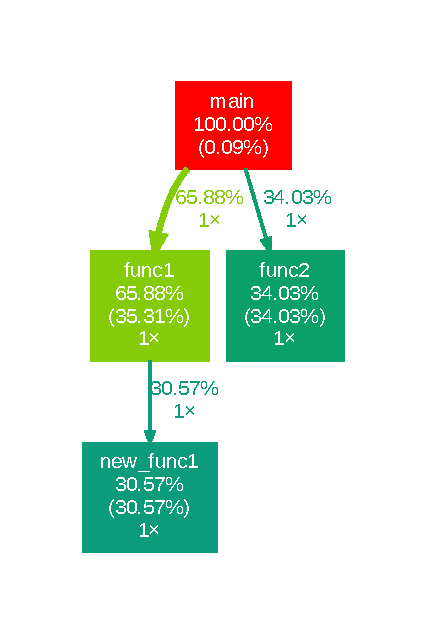
\includegraphics[height=0.6\textheight]{slides/sysdev-application-development/gprof2dot.pdf}\\
      {\small Generated with \href{https://github.com/jrfonseca/gprof2dot}{gprof2dot}}
    \end{center}
  \end{columns}
\end{frame}

\subsection{Memory debugging}

\begin{frame}{Valgrind}
  \begin{columns}[T]
    \column{0.8\textwidth}
    \url{https://valgrind.org/}
    \begin{itemize}
    \item {\em instrumentation framework for building dynamic analysis tools}
      \begin{itemize}
      \item detect many memory management and threading bugs
      \item profile programs
      \end{itemize}
    \item Supported architectures: x86, x86-64, ARMv7, arm64, mips32,
      s390, ppc32 and ppc64
    \item Very popular tool especially for debugging memory issues
    \item Runs your program on a synthetic CPU $\rightarrow$
      significant performance impact (100 x slower on SAMA5D3!),
      but very detailed instrumentation
    \item Runs on the target. Easy to build with Yocto Project
	  or Buildroot.
    \end{itemize}
    \column{0.2\textwidth}
    
\includegraphics[width=\textwidth]{common/valgrind1.png}
  \end{columns}
\end{frame}

\begin{frame}{Valgrind tools}
  \begin{itemize}
  \item {\em Memcheck}: detects memory-management problems
  \item {\em Cachegrind}: cache profiler, detailed simulation of the
    I1, D1 and L2 caches in your CPU and so can accurately pinpoint
    the sources of cache misses in your code
  \item {\em Callgrind}: extension to Cachegrind, provides extra
    information about call graphs
  \item {\em Massif}: performs detailed heap profiling by taking
    regular snapshots of a program's heap
  \item {\em Helgrind}: thread debugger which finds data races in
    multithreaded programs. Looks for memory locations accessed by
    multiple threads without locking.
  \item More at \url{https://valgrind.org/info/tools.html}
  \end{itemize}
\end{frame}

\begin{frame}[fragile]{Valgrind examples}
  \begin{itemize}
  \item {\em Memcheck}
    \begin{block}{}
      {\tiny
\begin{verbatim}
$ valgrind --leak-check=yes <program>
  ==19182== Invalid write of size 4
  ==19182==    at 0x804838F: f (example.c:6)
  ==19182==    by 0x80483AB: main (example.c:11)
  ==19182==  Address 0x1BA45050 is 0 bytes after a block of size 40 alloc'd
  ==19182==    at 0x1B8FF5CD: malloc (vg_replace_malloc.c:130)
  ==19182==    by 0x8048385: f (example.c:5)
  ==19182==    by 0x80483AB: main (example.c:11)
\end{verbatim}
      }
    \end{block}

  \item {\em Callgrind}
    \begin{block}{}
      {\tiny
\begin{verbatim}
$ valgrind --tool=callgrind --dump-instr=yes --simulate-cache=yes --collect-jumps=yes <program>
$ ls callgrind.out.*
callgrind.out.1234
$ callgrind_annotate callgrind.out.1234
\end{verbatim}
      }
    \end{block}
  \end{itemize}
\end{frame}

\begin{frame}{Kcachegrind - Visualizing Valgrind profiling data}
  \begin{center}
    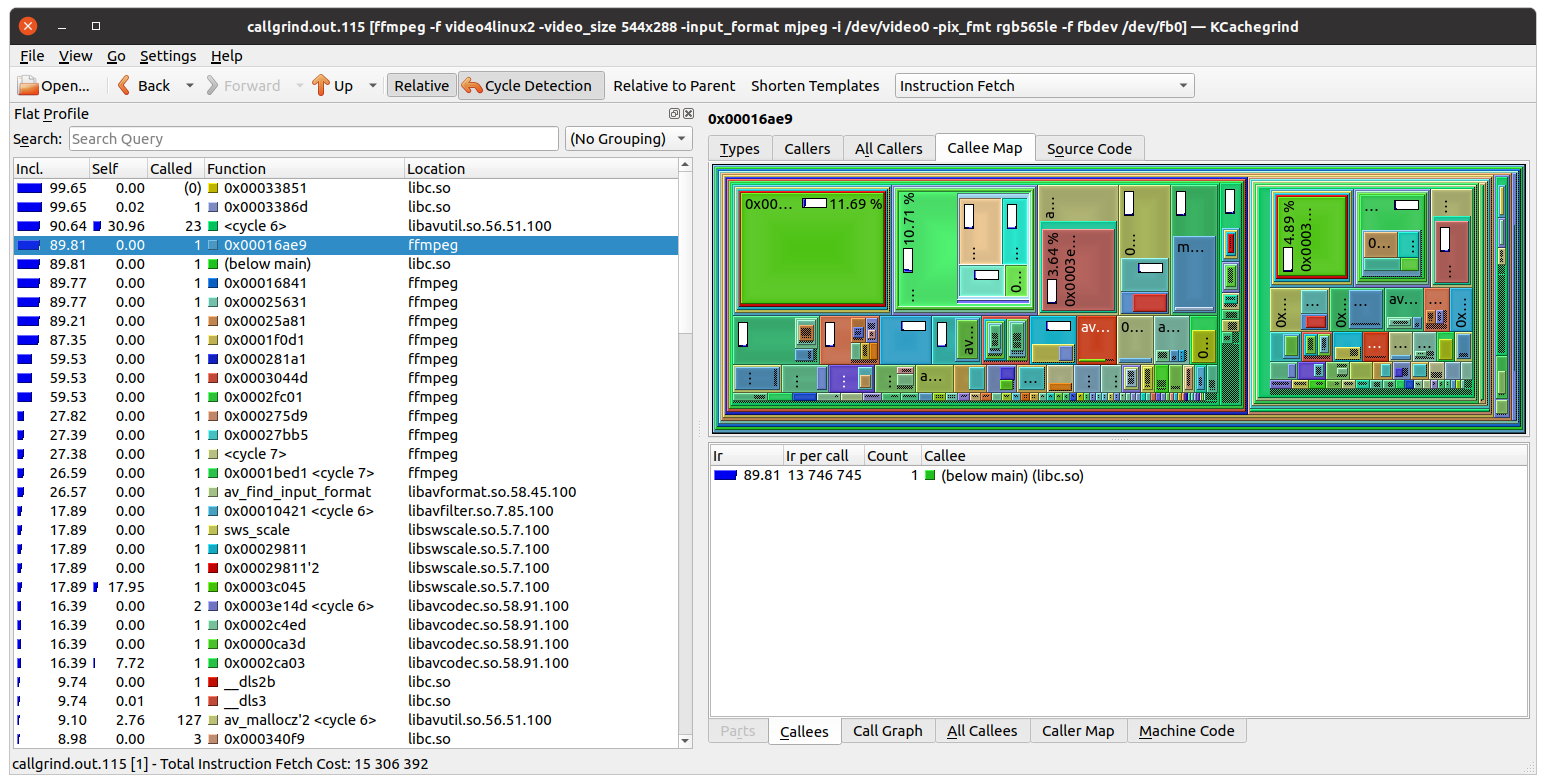
\includegraphics[height=0.8\textheight]{common/kcachegrind.png}
    \url{https://github.com/KDE/kcachegrind}
  \end{center}
\end{frame}


\begin{frame}{Debugging ressources}
  \begin{itemize}
  \item Brendan Gregg
    \href{https://www.brendangregg.com/systems-performance-2nd-edition-book.html}{Systems
      performance} book
  \item Brendan Gregg
    \href{https://www.brendangregg.com/linuxperf.html}{Linux
      Performance} page
  \item {\em Tools and Techniques to Debug an Embedded Linux System},
    talk from Sergio Prado,
    \href{https://www.youtube.com/watch?v=dgPkZnGuIMg}{video},
    \href{https://elinux.org/images/c/cf/Slides-debugging.pdf}{slides}
  \item {\em Tracing with Ftrace: Critical Tooling for Linux
      Development}, talk from Steven Rostedt,
    \href{https://www.youtube.com/watch?v=mlxqpNvfvEQ}{video}
  \item {\em Tutorial: Debugging Embedded Devices using GDB}, tutorial
    from Chris Simmonds,
    \href{https://www.youtube.com/watch?v=JGhAgd2a_Ck}{video}
  \end{itemize}
\end{frame}

\setuplabframe
{Application development and debugging}
{
  \begin{itemize}
  \item Creating an application that uses an I2C-connected joystick to
    control an audio player.
  \item Setting up an IDE to develop and remotely debug an
    application.
  \item Using {\em strace}, {\em ltrace}, {\em gdbserver} and {\em
      perf} to debug/investigate buggy applications on the embedded
    board.
  \end{itemize}
}

